\section{Test cases}

\begin{frame}{Academic Parts}

\begin{center}
\resizebox{0.4\linewidth}{!}{
\begin{tabular}[h]{@{}p{0.22\linewidth} p{0.22\linewidth}  p{0.22\linewidth}  p{0.22\linewidth} @{}} \toprule
{\bf Part} & {\bf Cellular}  & {\bf Graph} & {\bf Result} \\ \midrule  

\adjustbox{valign=t}{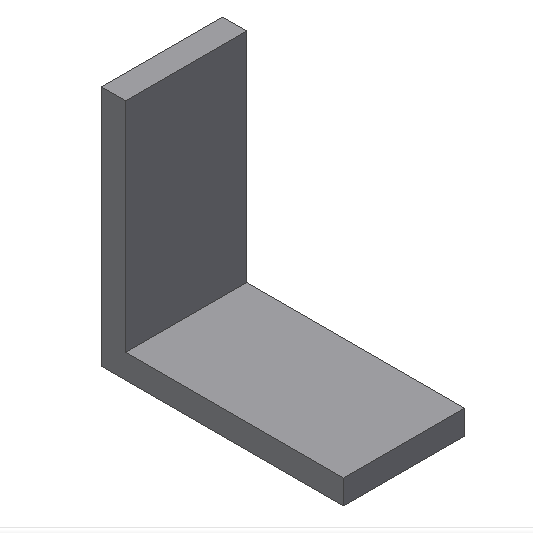
\includegraphics[width=\linewidth]{../Common/images/nonCellularL}}  &  
\adjustbox{valign=t}{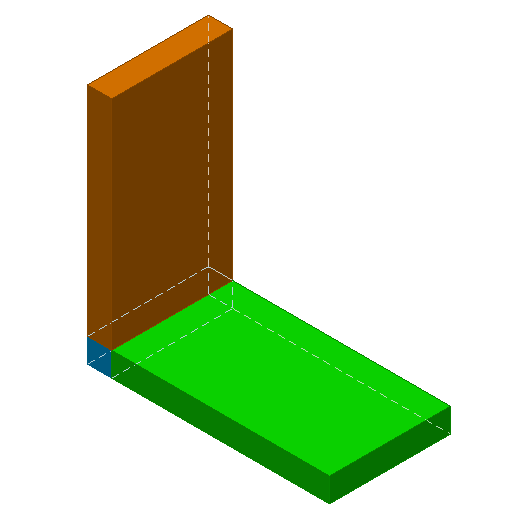
\includegraphics[width=\linewidth]{../Common/images/CellularL}}  &
\adjustbox{valign=t}{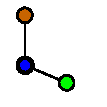
\includegraphics[width=\linewidth]{../Common/images/CellGraphL.pdf}} &  
\adjustbox{valign=t}{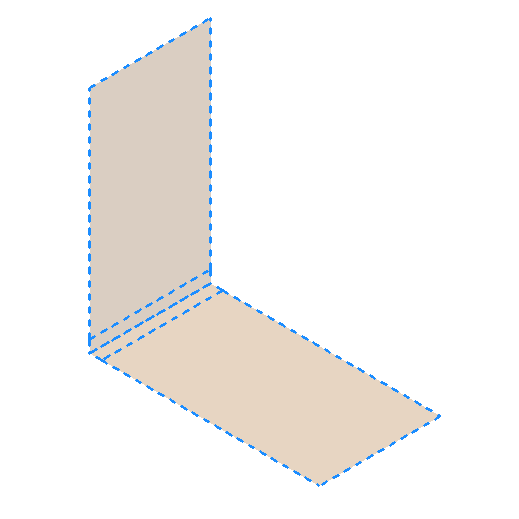
\includegraphics[width=\linewidth]{../Common/images/midsCellularL}} 
\\ \midrule

\adjustbox{valign=t}{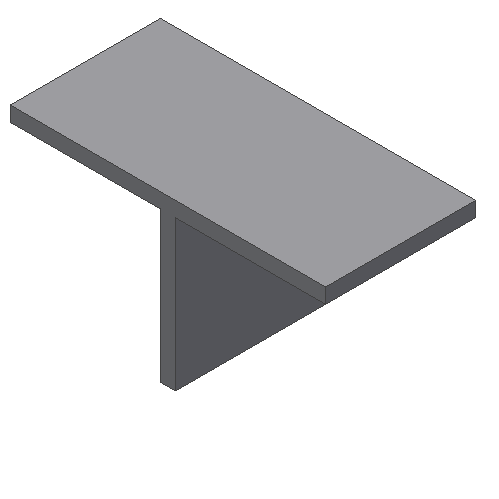
\includegraphics[width=\linewidth]{../Common/images/nonCellularT}}  &  
\adjustbox{valign=t}{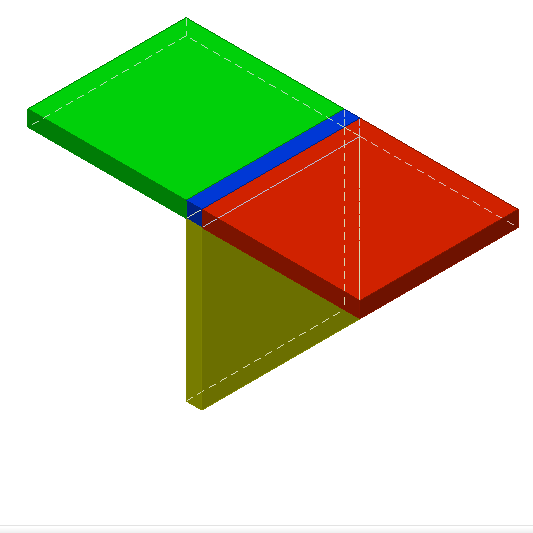
\includegraphics[width=\linewidth]{../Common/images/CellularT}}  &
\adjustbox{valign=t}{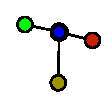
\includegraphics[width=\linewidth]{../Common/images/CellGraphT.pdf}} &  
\adjustbox{valign=t}{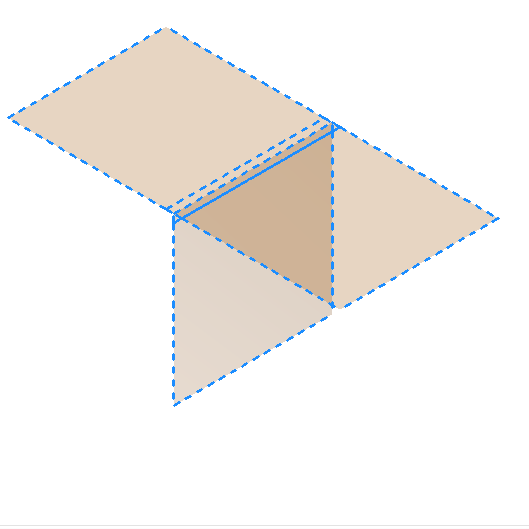
\includegraphics[width=\linewidth]{../Common/images/midsCellularT}} 
\\ \midrule

\adjustbox{valign=t}{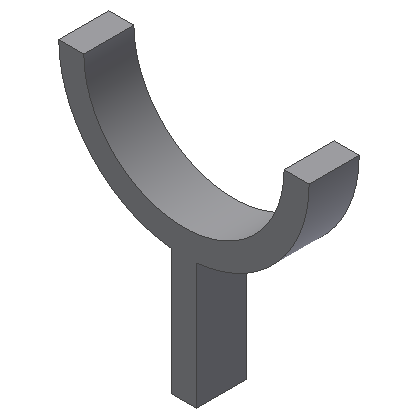
\includegraphics[width=\linewidth]{../Common/images/nonCellularCurvedY}}  &  
\adjustbox{valign=t}{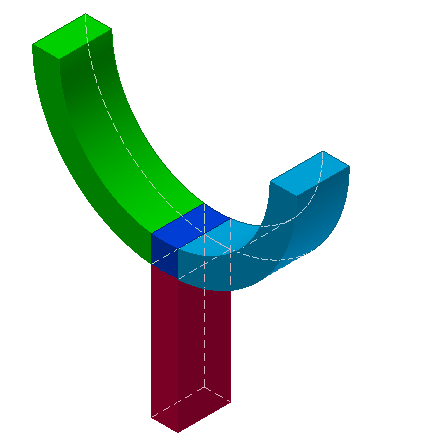
\includegraphics[width=\linewidth]{../Common/images/CellularCurvedY}}  &
\adjustbox{valign=t}{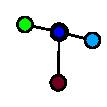
\includegraphics[width=\linewidth]{../Common/images/CellGraphY.pdf}} &  
\adjustbox{valign=t}{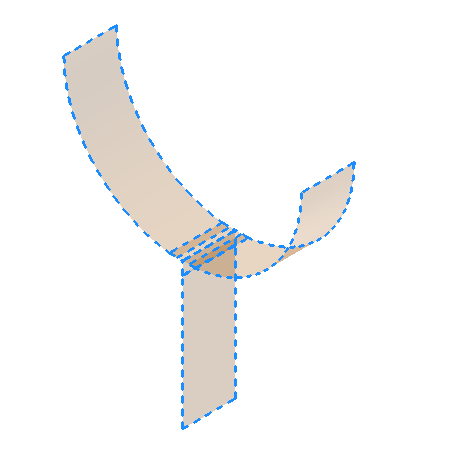
\includegraphics[width=\linewidth]{../Common/images/midsCellularCurvedY}} 
\\ \midrule


\adjustbox{valign=t}{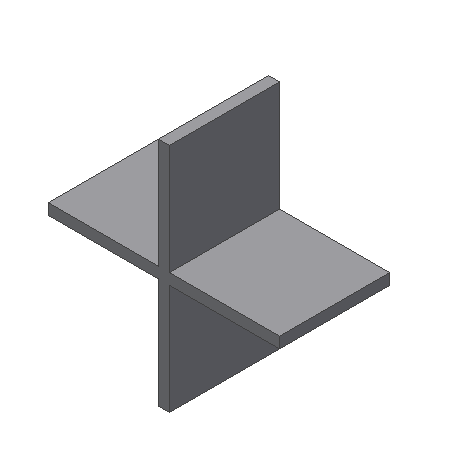
\includegraphics[width=\linewidth]{../Common/images/nonCellularPlus}}  &  
\adjustbox{valign=t}{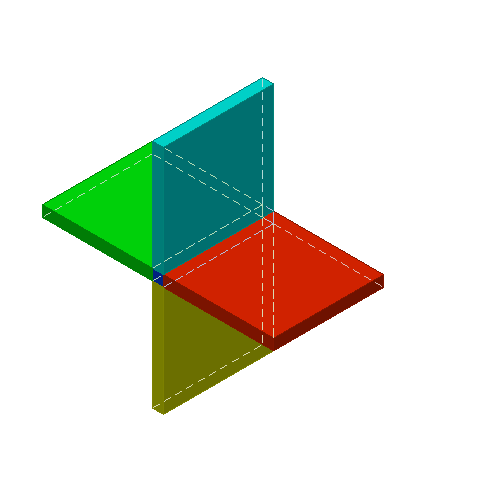
\includegraphics[width=\linewidth]{../Common/images/CellularPlus}}  &
\adjustbox{valign=t}{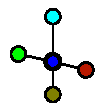
\includegraphics[width=\linewidth]{../Common/images/CellGraphPlus.pdf}} &  
\adjustbox{valign=t}{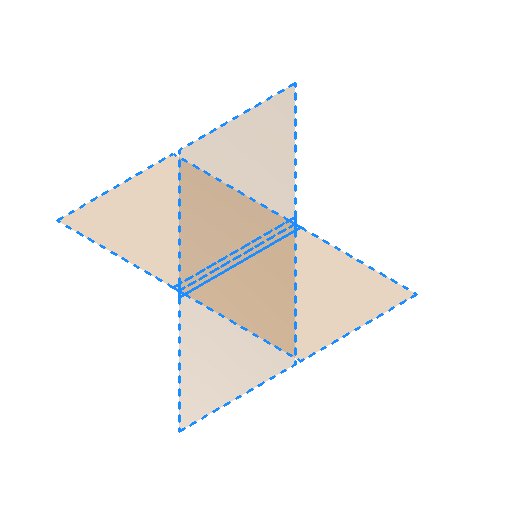
\includegraphics[width=\linewidth]{../Common/images/midsCellularPlus}} 
\\ \midrule

\adjustbox{valign=t}{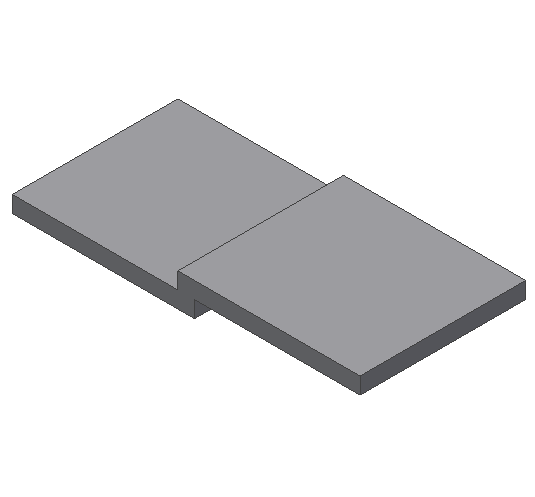
\includegraphics[width=\linewidth]{../Common/images/nonCellularOverlap}}  &  
\adjustbox{valign=t}{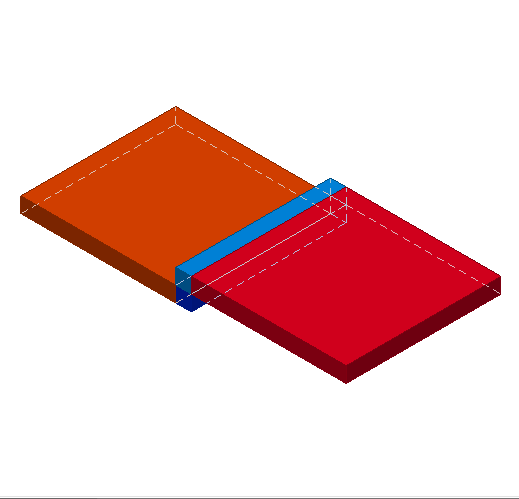
\includegraphics[width=\linewidth]{../Common/images/CellularOverlap}}  &
\adjustbox{valign=t}{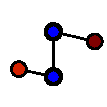
\includegraphics[width=\linewidth]{../Common/images/CellGraphOverlap.pdf}} &  
\adjustbox{valign=t}{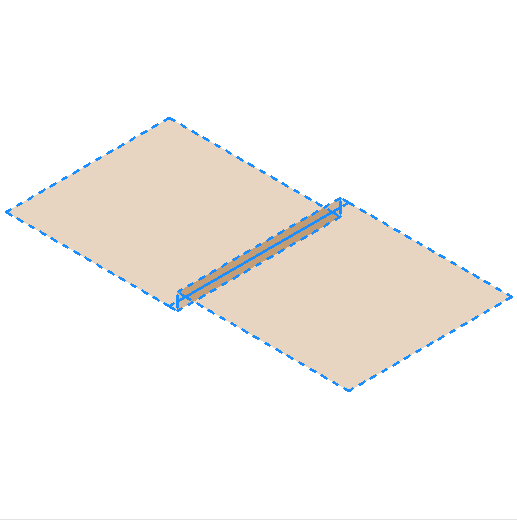
\includegraphics[width=\linewidth]{../Common/images/midsCellularOverlap}} 
\\ \midrule

\adjustbox{valign=t}{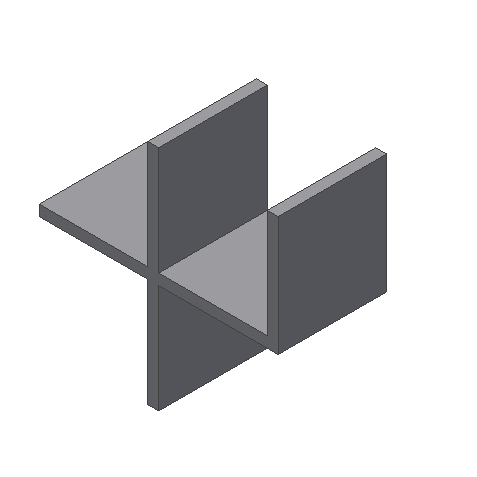
\includegraphics[width=\linewidth]{../Common/images/nonCellularZU}}  &  
\adjustbox{valign=t}{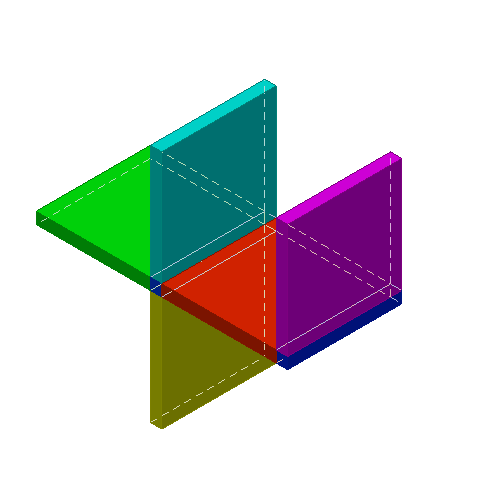
\includegraphics[width=\linewidth]{../Common/images/CellularZU}}  &
\adjustbox{valign=t}{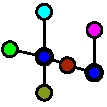
\includegraphics[width=\linewidth]{../Common/images/CellGraphZU.pdf}} &  
\adjustbox{valign=t}{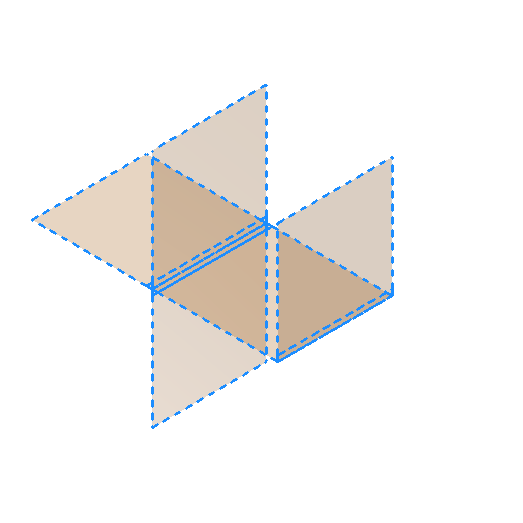
\includegraphics[width=\linewidth]{../Common/images/midsCellularZU}} 
\\ % \midrule

%\adjustbox{valign=t}{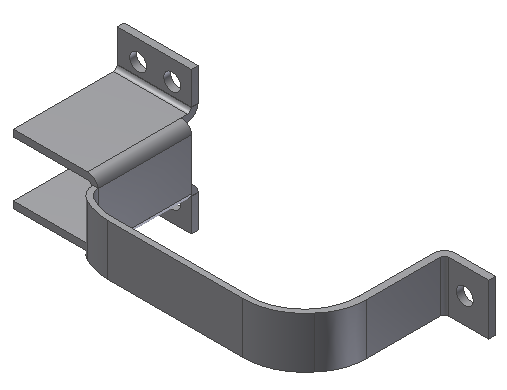
\includegraphics[width=\linewidth]{../Common/images/nonCellularBracket}}  &  
%\adjustbox{valign=t}{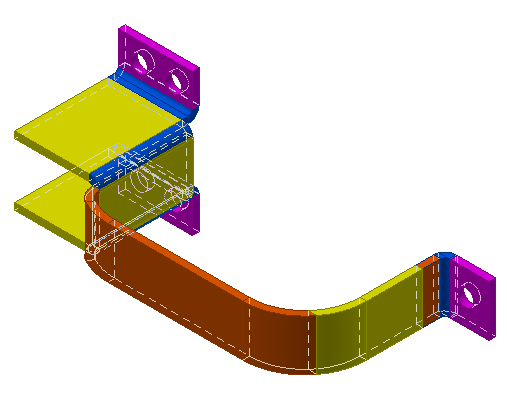
\includegraphics[width=\linewidth]{../Common/images/CellularBracket}}  &
%\adjustbox{valign=t}{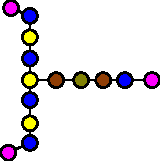
\includegraphics[width=\linewidth]{../Common/images/CellGraphBracket.pdf}} &  
%\adjustbox{valign=t}{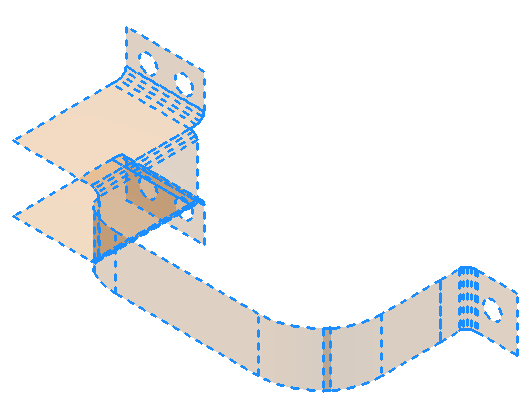
\includegraphics[width=\linewidth]{../Common/images/midsCellularBracket}} 
%\\ %\midrule
\bottomrule
\end{tabular}
}
\captionof{table}{Feature based Cellular Midsurface}\label{tbl_fbcm}
\end{center}

\end{frame}

%-------------------------------------------------------------------------------------

\begin{frame}{Practical Part}
The test-case is commonly used sheet metal bracket. It consists of various features such as face, flange, holes etc.

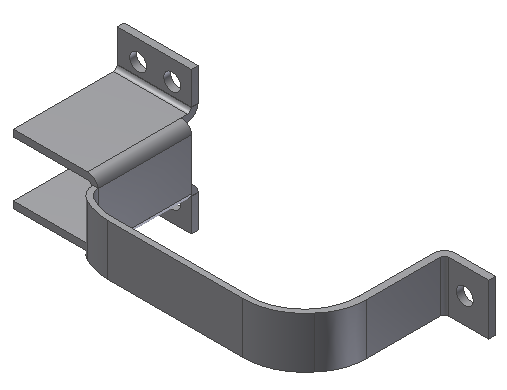
\includegraphics[width=0.8\linewidth]{../Common/images/nonCellularBracket}
\end{frame}

\begin{frame}{Cellular Decomposition}
The original part has been decmposed into non-verlapping cells. $iCell$s are marked with dark-blue color whereas $sCells$ are shown in various colors.

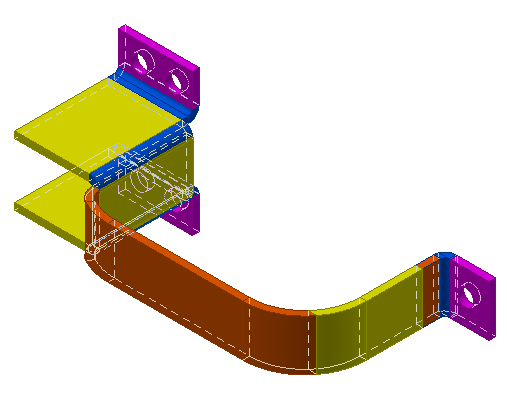
\includegraphics[width=0.8\linewidth]{../Common/images/CellularBracket}
\end{frame}

\begin{frame}{Cellular Graph}
The cells are composed in the form of a cellular graph where nodes represent cells and edges represent connections.

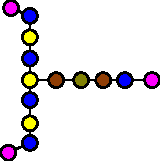
\includegraphics[width=0.6\linewidth]{../Common/images/CellGraphBracket.pdf}
\end{frame}

\begin{frame}{Midsurface}
The output shows computationn of well connected midsurface.

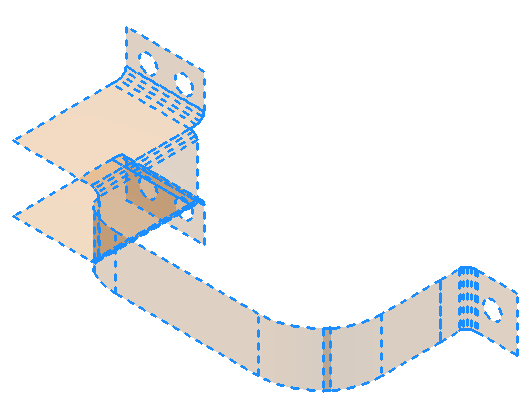
\includegraphics[width=0.8\linewidth]{../Common/images/midsCellularBracket}
\end{frame}
